% write_head_timing.tex — Williams Tube Write Head Timing Diagram
% Shows parameter states during a typical screen transition:
%   CLEAR → MACRO stamp → TEXT writes → VQ bitmap writes

\newcommand{\wttbus}[5]{%
  % Bus value segment: #1=x1, #2=x2, #3=y-center, #4=label, #5=fill
  \fill[#5] ({#1+0.12},{#3+0.2}) -- ({#2-0.12},{#3+0.2}) -- ({#2},{#3})
    -- ({#2-0.12},{#3-0.2}) -- ({#1+0.12},{#3-0.2}) -- ({#1},{#3}) -- cycle;
  \draw ({#1},{#3}) -- ({#1+0.12},{#3+0.2}) -- ({#2-0.12},{#3+0.2})
    -- ({#2},{#3}) -- ({#2-0.12},{#3-0.2}) -- ({#1+0.12},{#3-0.2}) -- cycle;
  \node[font=\tiny\ttfamily] at ({(#1+#2)/2},{#3}) {#4};%
}
\newcommand{\wttstl}[3]{%
  % Settle/unknown segment: #1=x1, #2=x2, #3=y-center
  \fill[gray!10] ({#1},{#3-0.2}) rectangle ({#2},{#3+0.2});
  \draw ({#1},{#3+0.2}) -- ({#2},{#3+0.2});
  \draw ({#1},{#3-0.2}) -- ({#2},{#3-0.2});
  \draw[gray!40] ({#1},{#3+0.2}) -- ({#2},{#3-0.2});
  \draw[gray!40] ({#1},{#3-0.2}) -- ({#2},{#3+0.2});%
}

\begin{figure}[H]
\centering
\resizebox{0.95\textwidth}{!}{%
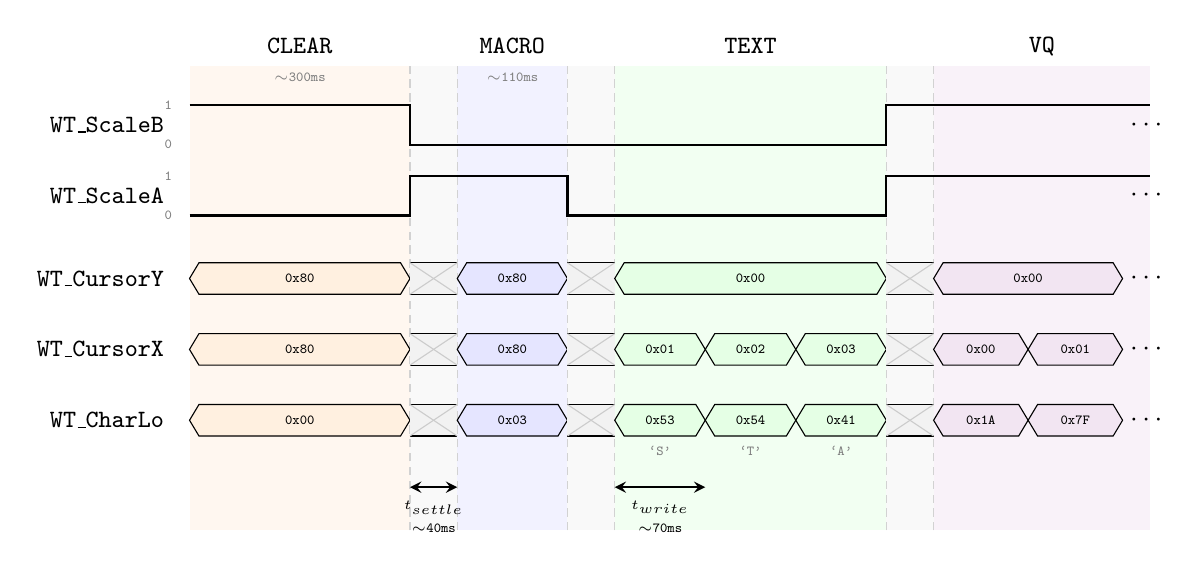
\begin{tikzpicture}[y=1cm, >=stealth]

% ================================================================
% Time positions (in cm):
%   CLEAR:   0.0 -- 2.8
%   Settle:  2.8 -- 3.4
%   MACRO:   3.4 -- 4.8
%   Settle:  4.8 -- 5.4
%   TEXT:    5.4 -- 8.85  (3 chars: 5.4--6.55, 6.55--7.7, 7.7--8.85)
%   Settle:  8.85 -- 9.45
%   VQ:      9.45 -- 11.85 (2 tiles: 9.45--10.65, 10.65--11.85)
%   Dots:    ~12.1
% ================================================================

% ================================================================
% Phase background shading
% ================================================================
\fill[orange!6]  (0, -0.5) rectangle (2.8, 5.4);
\fill[gray!5]    (2.8, -0.5) rectangle (3.4, 5.4);
\fill[blue!5]    (3.4, -0.5) rectangle (4.8, 5.4);
\fill[gray!5]    (4.8, -0.5) rectangle (5.4, 5.4);
\fill[green!5]   (5.4, -0.5) rectangle (8.85, 5.4);
\fill[gray!5]    (8.85, -0.5) rectangle (9.45, 5.4);
\fill[violet!5]  (9.45, -0.5) rectangle (12.2, 5.4);

% ================================================================
% Phase separator lines
% ================================================================
\foreach \tx in {2.8, 3.4, 4.8, 5.4, 8.85, 9.45} {
  \draw[densely dashed, gray!35] (\tx, -0.5) -- (\tx, 5.4);
}

% ================================================================
% Phase labels (top)
% ================================================================
\node[font=\small\ttfamily\bfseries] at (1.4, 5.65) {CLEAR};
\node[font=\small\ttfamily\bfseries] at (4.1, 5.65) {MACRO};
\node[font=\small\ttfamily\bfseries] at (7.125, 5.65) {TEXT};
\node[font=\small\ttfamily\bfseries] at (10.825, 5.65) {VQ};
\node[font=\tiny\ttfamily, gray] at (1.4, 5.25) {$\sim$300ms};
\node[font=\tiny\ttfamily, gray] at (4.1, 5.25) {$\sim$110ms};

% ================================================================
% Signal: WT_ScaleB — low=4.4, high=4.9
% CLEAR(H) → MACRO(L) → TEXT(L) → VQ(H)
% ================================================================
\node[font=\small\ttfamily, anchor=east] at (-0.2, 4.65) {WT\_ScaleB};
\draw[thick] (0, 4.9) -- (2.8, 4.9)
  -- (2.8, 4.4) -- (8.85, 4.4)
  -- (8.85, 4.9) -- (12.2, 4.9);
% LOW reference
\draw[dotted, gray!25] (2.8, 4.4) -- (2.8, 4.4);

% ================================================================
% Signal: WT_ScaleA — low=3.5, high=4.0
% CLEAR(L) → MACRO(H) → TEXT(L) → VQ(H)
% ================================================================
\node[font=\small\ttfamily, anchor=east] at (-0.2, 3.75) {WT\_ScaleA};
\draw[thick] (0, 3.5) -- (2.8, 3.5)
  -- (2.8, 4.0) -- (4.8, 4.0)
  -- (4.8, 3.5) -- (8.85, 3.5)
  -- (8.85, 4.0) -- (12.2, 4.0);

% HIGH / LOW annotations
\node[font=\tiny\ttfamily, gray, anchor=east] at (-0.1, 4.9) {1};
\node[font=\tiny\ttfamily, gray, anchor=east] at (-0.1, 4.4) {0};
\node[font=\tiny\ttfamily, gray, anchor=east] at (-0.1, 4.0) {1};
\node[font=\tiny\ttfamily, gray, anchor=east] at (-0.1, 3.5) {0};

% ================================================================
% Signal: WT_CursorY — bus, center=2.7
% CLEAR/MACRO: 0x80 (centered), TEXT/VQ: 0x00 (row/tile 0)
% ================================================================
\node[font=\small\ttfamily, anchor=east] at (-0.2, 2.7) {WT\_CursorY};
\wttbus{0}{2.8}{2.7}{0x80}{orange!12}
\wttstl{2.8}{3.4}{2.7}
\wttbus{3.4}{4.8}{2.7}{0x80}{blue!10}
\wttstl{4.8}{5.4}{2.7}
\wttbus{5.4}{8.85}{2.7}{0x00}{green!10}
\wttstl{8.85}{9.45}{2.7}
\wttbus{9.45}{11.85}{2.7}{0x00}{violet!10}

% ================================================================
% Signal: WT_CursorX — bus, center=1.8
% CLEAR/MACRO: 0x80, TEXT: steps through columns, VQ: steps through tiles
% ================================================================
\node[font=\small\ttfamily, anchor=east] at (-0.2, 1.8) {WT\_CursorX};
\wttbus{0}{2.8}{1.8}{0x80}{orange!12}
\wttstl{2.8}{3.4}{1.8}
\wttbus{3.4}{4.8}{1.8}{0x80}{blue!10}
\wttstl{4.8}{5.4}{1.8}
\wttbus{5.4}{6.55}{1.8}{0x01}{green!10}
\wttbus{6.55}{7.7}{1.8}{0x02}{green!10}
\wttbus{7.7}{8.85}{1.8}{0x03}{green!10}
\wttstl{8.85}{9.45}{1.8}
\wttbus{9.45}{10.65}{1.8}{0x00}{violet!10}
\wttbus{10.65}{11.85}{1.8}{0x01}{violet!10}

% ================================================================
% Signal: WT_CharLo — bus, center=0.9
% CLEAR: 0x00, MACRO: glyph index, TEXT: ASCII, VQ: codebook index
% ================================================================
\node[font=\small\ttfamily, anchor=east] at (-0.2, 0.9) {WT\_CharLo};
\wttbus{0}{2.8}{0.9}{0x00}{orange!12}
\wttstl{2.8}{3.4}{0.9}
\wttbus{3.4}{4.8}{0.9}{0x03}{blue!10}
\wttstl{4.8}{5.4}{0.9}
\wttbus{5.4}{6.55}{0.9}{0x53}{green!10}
\wttbus{6.55}{7.7}{0.9}{0x54}{green!10}
\wttbus{7.7}{8.85}{0.9}{0x41}{green!10}
\wttstl{8.85}{9.45}{0.9}
\wttbus{9.45}{10.65}{0.9}{0x1A}{violet!10}
\wttbus{10.65}{11.85}{0.9}{0x7F}{violet!10}

% ASCII character annotations below CharLo during TEXT phase
\node[font=\tiny, gray] at ({(5.4+6.55)/2}, 0.5) {\texttt{`S'}};
\node[font=\tiny, gray] at ({(6.55+7.7)/2}, 0.5) {\texttt{`T'}};
\node[font=\tiny, gray] at ({(7.7+8.85)/2}, 0.5) {\texttt{`A'}};

% ================================================================
% Continuation dots
% ================================================================
\foreach \yy in {4.65, 3.75, 2.7, 1.8, 0.9} {
  \node[font=\normalsize] at (12.15, \yy) {$\cdots$};
}

% ================================================================
% Timing annotations
% ================================================================
% Settle delay
\draw[<->, thick] (2.8, 0.05) -- (3.4, 0.05);
\node[font=\tiny\ttfamily, below] at (3.1, 0.0) {$t_{settle}$};
\node[font=\tiny\ttfamily, below] at (3.1, -0.3) {$\sim$40ms};

% Write delay (one character)
\draw[<->, thick] (5.4, 0.05) -- (6.55, 0.05);
\node[font=\tiny\ttfamily, below] at (5.975, 0.0) {$t_{write}$};
\node[font=\tiny\ttfamily, below] at (5.975, -0.3) {$\sim$70ms};

\end{tikzpicture}%
}

\par\vspace{0.3em}
{\footnotesize\ttfamily Figure 3: Write head parameter timing during a typical screen transition.
WT\_ScaleA and WT\_ScaleB select the write mode (see Section~\ref{sec:writemodes}).
WT\_CursorX/Y position the write head. WT\_CharLo selects the glyph, macro index,
or VQ codebook entry. Hatched regions indicate settle delays between mode changes.
TEXT values shown: 0x53=`S', 0x54=`T', 0x41=`A'.}
\end{figure}
